\documentclass[12pt]{article}
\usepackage{amsmath,amssymb,amsthm}
\usepackage[margin=1in]{geometry}
\usepackage{graphicx,enumitem}
\usepackage{tikz,fancyhdr}
\usepackage[labelfont=bf]{caption}

\pagestyle{fancy}
\fancyhf{}
\chead{PROBLEM SET 4}
\rhead{Elliot Ahn}
\lhead{Machine Learning}
\rfoot{\thepage}

\setlength{\headheight}{15pt}
\renewcommand{\footrulewidth}{0.5pt}

\newcommand{\dvc}{{d_{\text{VC}}}}

\begin{document}

\begin{enumerate}[leftmargin=*]
\item (d)
\[ 0.05 = \delta = 4 m_{\mathcal H}(2N) \exp \left(- \frac{1}{8} \epsilon^2 N \right) \]
Making the large sample approximation
\[ m_{\mathcal H} (N) \approx N^\dvc \]
So
\[ 0.05 = \delta \approx 4 (2 N)^\dvc \exp \left( - \frac{1}{8} \epsilon^2 N \right)\]
Solving for $N$ must be done numerically, and this gives
\[ N \approx 453,000 \]
\item (d)
\begin{figure}[h!]
\centering
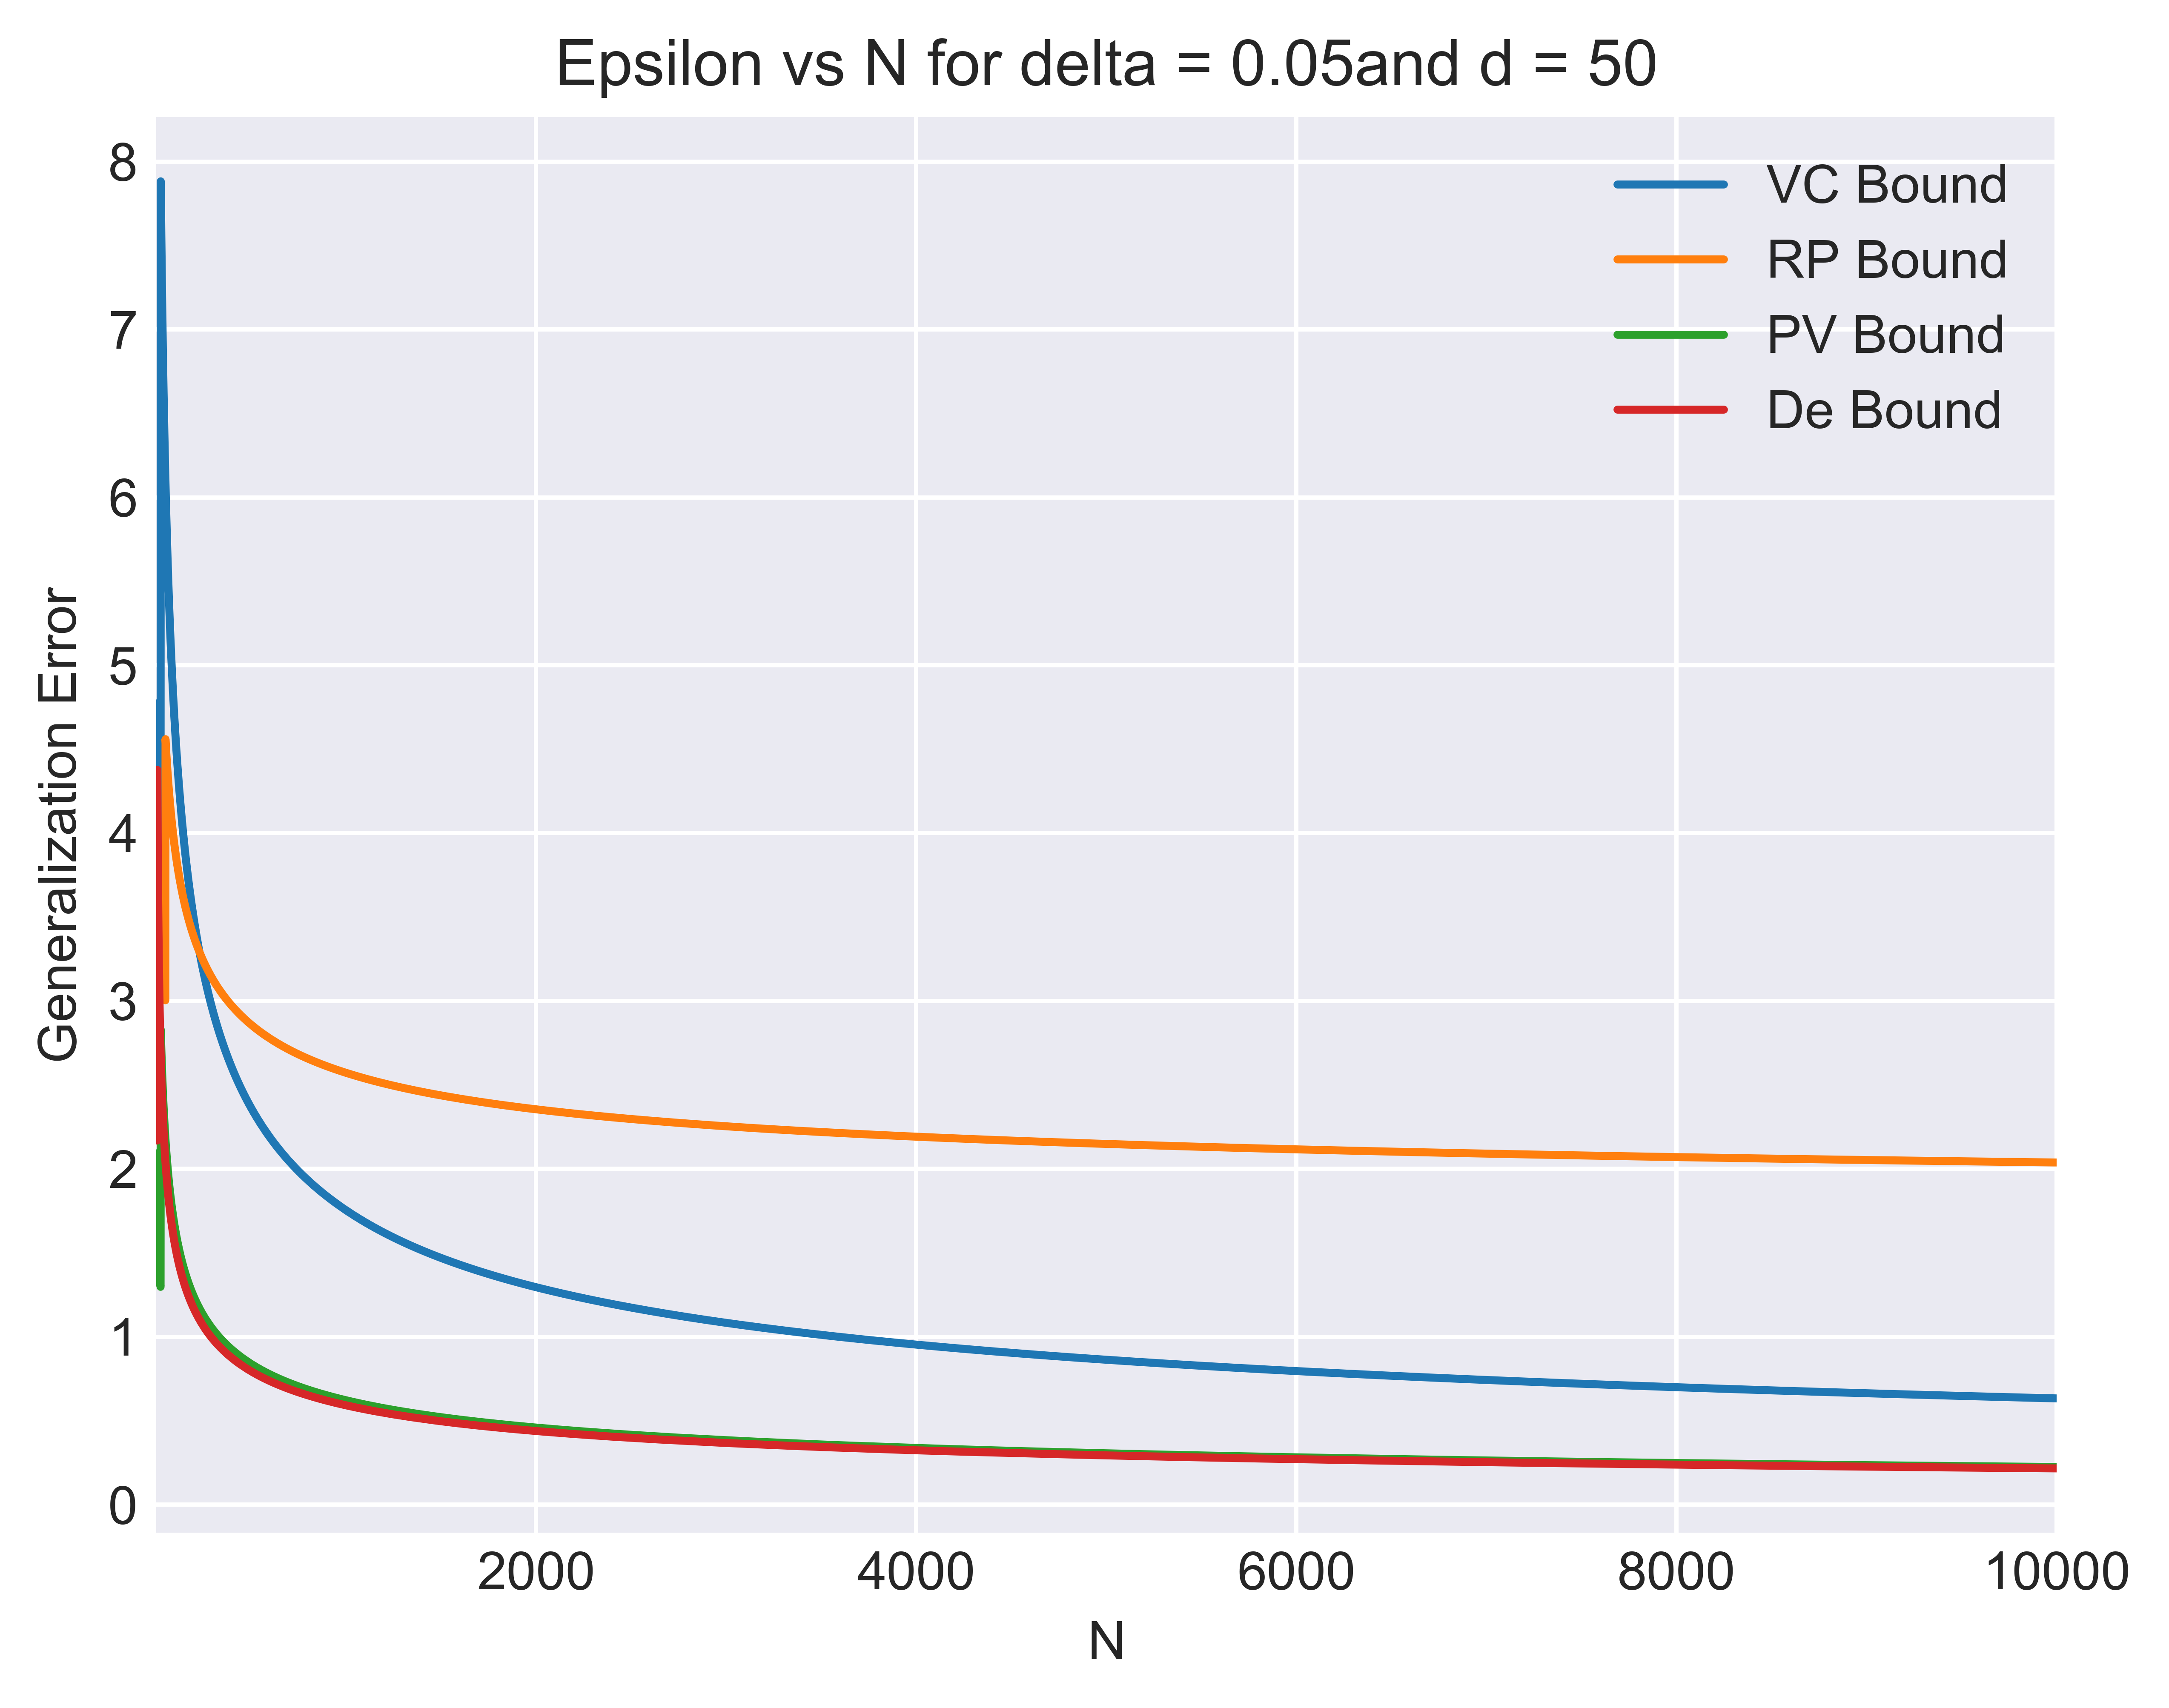
\includegraphics[scale=0.55]{epsilonvsN.png}
\end{figure}
\item (c)
\begin{figure}[h!]
\centering
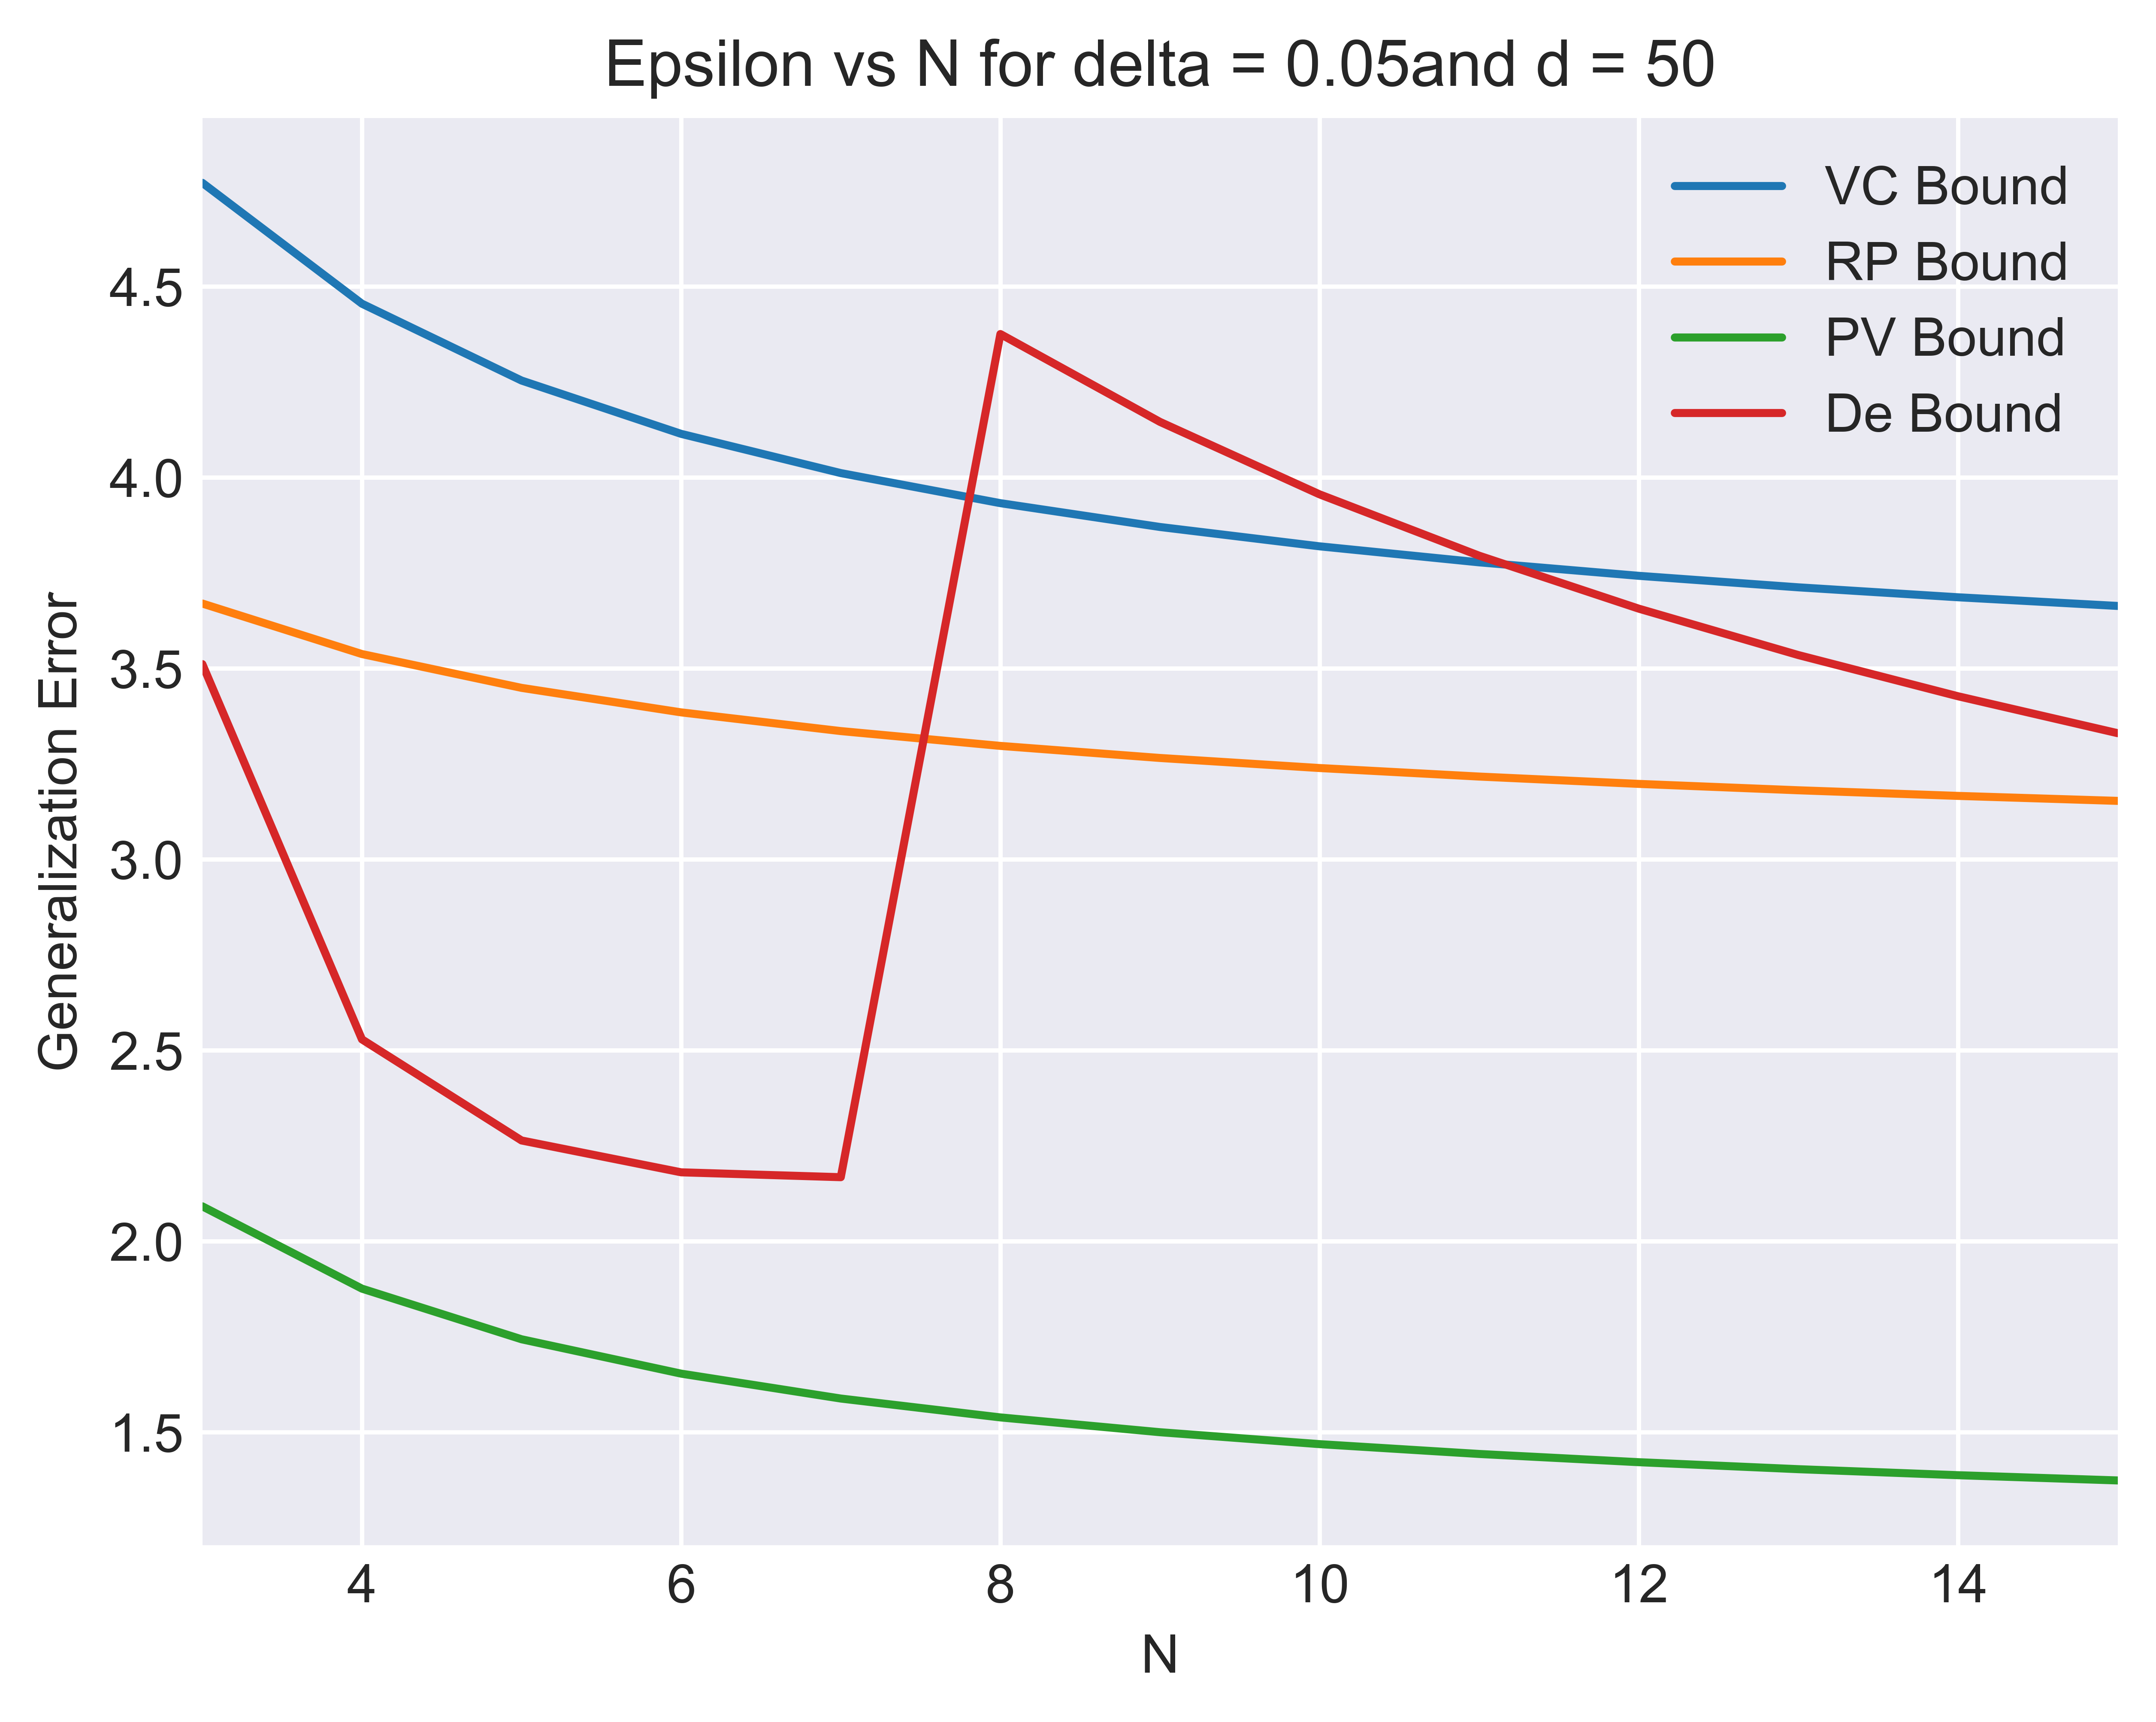
\includegraphics[scale=0.55]{epsilonvssmallN.png}
\end{figure}
\item (e) We can get the expected value $\hat a$ by running a linear regression multiple times and averaging out, or we can calculate the value
\[ \hat a = \frac{1}{4}\int_{-1}^1 \int_{-1}^1 dx_1 \, dx_2 \frac{x_1 \sin \pi x_1 + x_2 \sin \pi x_2}{x_1^2 + x_2^2} = \frac{1}{2} \int_{-1}^1 \int_0^1 dx_1 \, dx_2 \frac{x_1 \sin \pi x_1 + x_2 \sin \pi x_2}{x_1^2 + x_2^2} \]
\[ \hat a \approx 1.43 \]
\[ \text{Var} \, \hat a = \frac{1}{2} \int_{-1}^1 \int_{0}^1 d x_1 \, dx_2 \left( \frac{x_1 \sin \pi x_1 + x_2 \sin \pi x_2}{x_1^2 + x_2^2} - \hat a \right)^2 = 0.71 \]
\begin{figure}[h!]
\centering
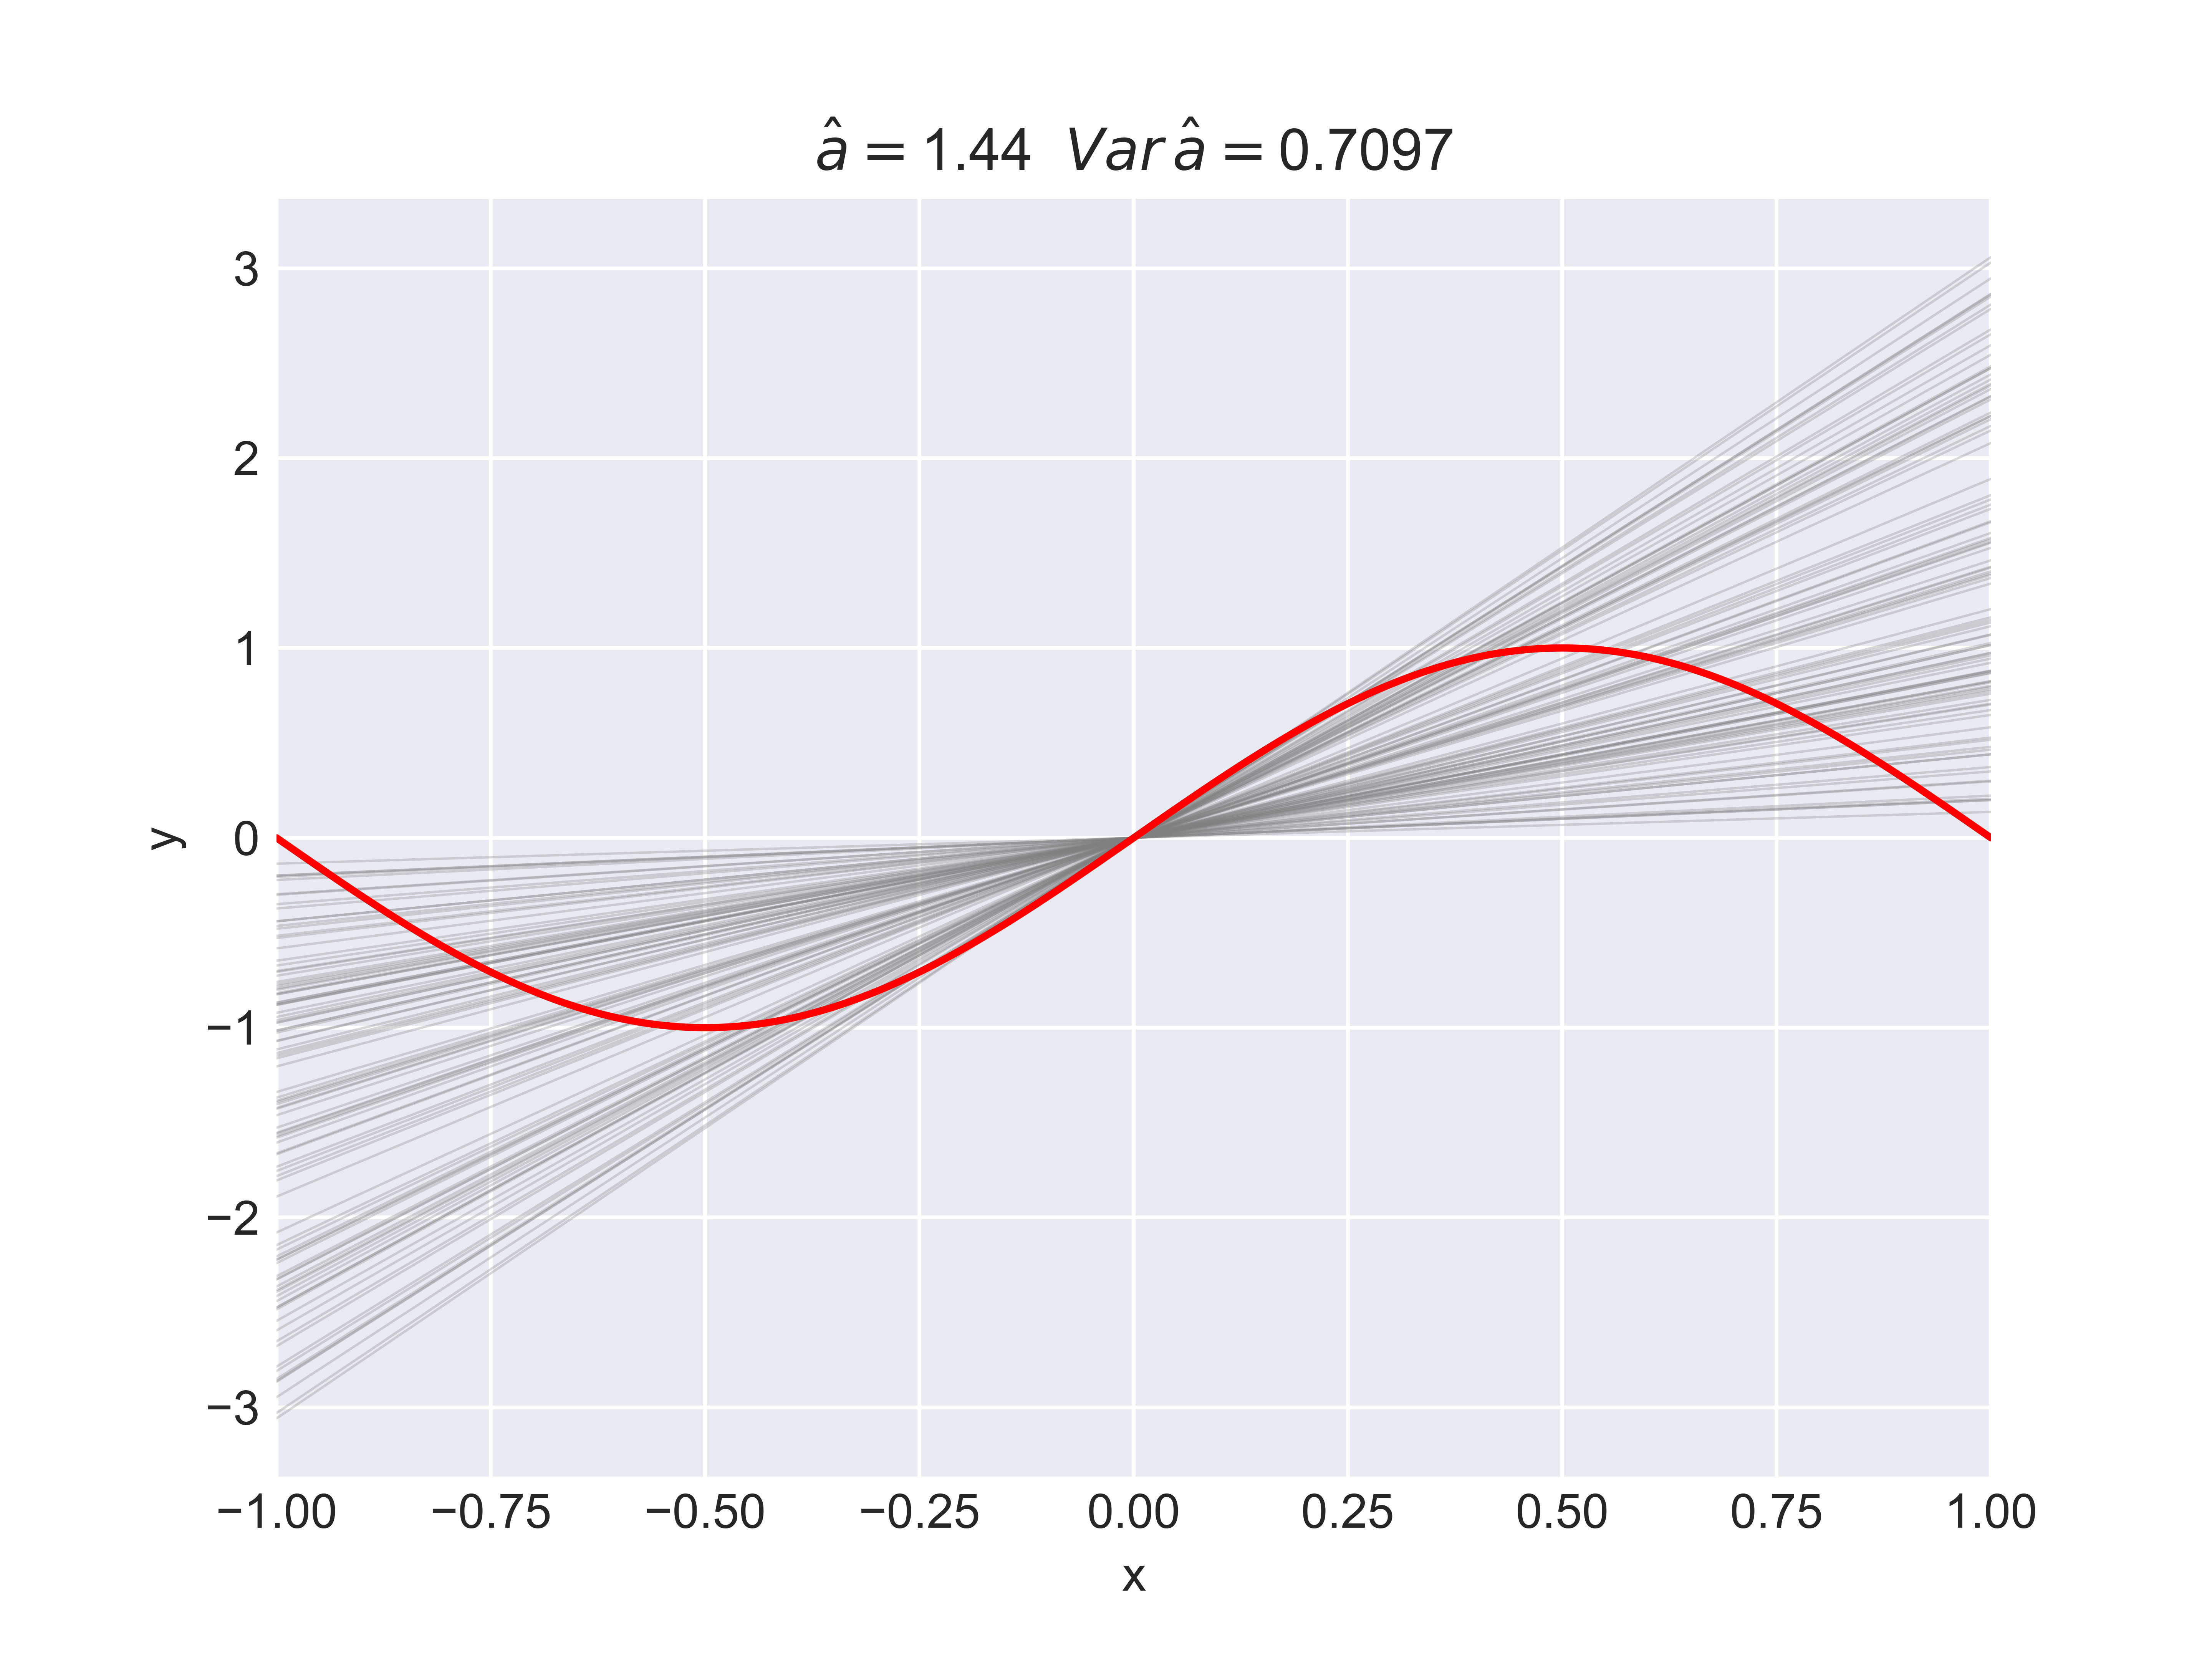
\includegraphics[scale=0.55]{SinLinReg.png}
\end{figure}
\item (b) The bias is given by
\[ \text{bias} = \frac{1}{2} \int_{-1}^1 dx \, \left( \sin \pi x - \hat a x \right)^2 = 0.27 \]
\item (d) The variance of $\hat a$ is given in problem 4.
\[ \text{Var} = \frac{1}{3} \text{Var} \, \hat a = 0.24 \]
\item (b)
\begin{figure}[h!]
\centering
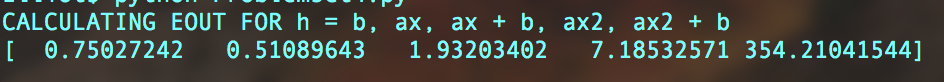
\includegraphics[scale=0.8]{eoutfig.png}
\end{figure}
\item (c) Assume that $k$ is the VC dimension, we have
\[ 2^k = m_{\mathcal H} (k) = 2 \cdot 2^{k-1} - \binom{k-1}{q} = m_{\mathcal H}(k)- \binom{k-1}{q} \]
which implies that $q = k$. This implies that that the VC dimension is $q$.
\item (b) We can think of the size of
\[ \bigcap_{k=1}^K \mathcal H_k \]
being at most the smallest set. So
\[ 0 \leq d_{\text{VC}} \left(\bigcap_{k=1}^K \mathcal H_k \right) \leq \text{min} \{ d_{\text{VC}} (\mathcal H_k)\}_{k=1}^K \]
\item Same as the previous problem, the lower bound is bound by the maximum size, or the VC dimension of the highest VC-dimensional hypothesis set. Now consider two hypothesis sets $\mathcal H_1$ and $\mathcal H_2$ with VC dimension $d_1$ and $d_2$ respectively. Then
\[ m_{\mathcal H_1 \cup \mathcal H_2}(N) \leq \sum_{i = 0}^{d_1} \binom{N}{i} + \sum_{i = 0}^{d_2} \binom{N}{i}, \]
and using the fact that
\[ \binom{N}{i} = \binom{N}{N - i} \]
yields
\[ m_{\mathcal H_1 \cup \mathcal H_2}(N) \leq \sum_{i=0}^{d_1} \binom{N}{i} + \sum_{i=0}^{d_2} \binom{N}{N - i} = \sum_{i=0}^{d_1} \binom{N}{i} + \sum_{i = N - d_2}^N \binom{N}{i} \]
If $N - d_2 > d_1 + 1$, that is $N \geq d_1 + d_2 + 2$, then
\[ m_{\mathcal H_1 \cup \mathcal H_2}(N) \leq \sum_{i=0}^N \binom{N}{i} - \binom{N}{d_1 + 1} = 2^N - \binom{N}{d_1 + 1} < 2^N \]
so the VC dimension of the union set is at most $d_1 + d_2 + 1$.

Now we can prove inductively for many sets $\mathcal H_1, \cdots, \mathcal H_k$ that the VC dimension is
\[ k - 1 + \sum_{i=0}^k d_i. \]
\end{enumerate}

\end{document}